\documentclass[11pt, twocolumn, landscape]{article}
\usepackage[utf8]{inputenc}
\usepackage[T1]{fontenc}
\usepackage[francais]{babel}
\usepackage{amsmath}
\usepackage{graphicx}
\usepackage{color}
\usepackage{pdfpages} 
\usepackage{listings}
\usepackage{graphicx}
\usepackage{hyperref}
\usepackage{amsthm}
\usepackage{amssymb}
\usepackage{mathrsfs}
\usepackage{moreverb}
\usepackage{titletoc}
\usepackage{lmodern}
\usepackage{cubeDrawing}
\usepackage{lipsum}
\usepackage{bbold}

\definecolor{oxf}{RGB}{0, 33, 71}
\definecolor{or}{RGB}{239, 155, 15}
\definecolor{vert}{RGB}{135,167,103}
\definecolor{rouge}{RGB}{181,39,39}
\definecolor{violet}{RGB}{64,9,90}


\newcommand{\oxf}[1]{\textcolor{oxf}{#1}}

%Macros pour modifier la table des matières
\hypersetup{colorlinks=true, urlcolor=bleu, linkcolor=black}
\usepackage{hyperref}

\titlecontents{chapter}[20pt]% 103
   {\addvspace{1pc}\normalfont\sffamily\bfseries\large} 
            {\contentslabel[\thecontentslabel]{20pt}}{}{\hfill\contentspage}[] 
\titlecontents{section}[40pt]% 
   {\addvspace{0.6pc}\normalfont\sffamily} 
            {\contentslabel[\thecontentslabel]{25pt}}{}{\dotfill\contentspage}[] 
\titlecontents{subsection}[60pt]% 
   {\addvspace{0.3pc}\normalfont\sffamily} 
            {\contentslabel[\thecontentslabel]{25pt}}{}{\dotfill\contentspage}[]                            
\titlecontents*{subsubsection}[60pt]% 
   {\filright\normalfont\sffamily\footnotesize}{}{}{}[~{–}\ ][] 
\setcounter{tocdepth}{2}

\makeatletter\@addtoreset{section}{part}
\makeatother



%Page de garde
\makeatletter

\def\graphic#1{\def\@graphic{#1}}
\graphic{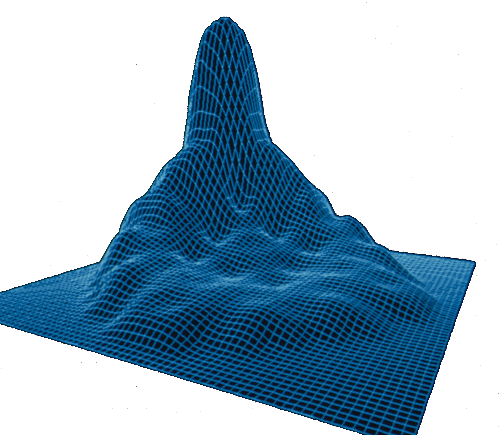
\includegraphics[scale=0.4]{logo.png}}
\def\clap#1{\hbox to 0pt{\hss #1\hss}}%
\def\ligne#1{%
\hbox to \hsize{%
\vbox{\centering #1}}}%
\def\haut#1#2#3{%
\hbox to \hsize{%
\rlap{\vtop{\raggedright #1}}%
\hss
\clap{\vtop{\centering #2}}%
\hss
\llap{\vtop{\raggedleft #3}}}}%
\def\bas#1#2#3{%
\hbox to \hsize{%
\rlap{\vbox{\raggedright #1}}%
\hss
\clap{\vbox{\centering #2}}%
\hss
\llap{\vbox{\raggedleft #3}}}}%
\def\maketitle{%
\thispagestyle{empty}\vbox to \vsize{%
\begin{tikzpicture}[remember picture,overlay]
\coordinate [below=2.5cm] (midpoint) at (current page.north);
\node [name=colourbar,
anchor=base,
fill=oxf,
minimum width=\paperwidth,
minimum height=1cm] at (midpoint){};
\node [
fill=oxf,
text = white,
xshift=2cm] at (midpoint){\Large{\textsf{Institut National des Sciences Appliquées de Rouen}}};
% Define the point where the logo will go
\coordinate [right=4cm] (logo) at (colourbar.west);
% Set coordinate system origin
\begin{scope}[shift=(logo)]
% Draw the outline
%\filldraw [white,draw=oxf] (2.3,0.85) -- (-2,0.85) -- (-2.8,-0.85) -- (2.3,-0.85) --cycle;
\filldraw [white,draw=oxf] (2.3,0.85) -- (-2.5,0.85) -- (-2.5,-0.85) -- (2.3,-0.85) --cycle;
\filldraw [oxf,draw=oxf] (-10,-24) -- (30,-24) -- (30,-23) -- (-10,-23) --cycle;
% Include the logo
\node {\includegraphics[width=4cm]{logoINSAdeRouen.jpg}};
\end{scope}
\end{tikzpicture}
\vspace{3cm}
%\usefont{OT1}{phv}{m}{n}
\begin{center}
\textbf{\huge \@title }
\end{center}
\vspace{1cm}
\par
\hrule height 4pt
\par
\vspace{0.5cm}
\begin{center}
\Large \@author
\par
\end{center}
\vfill
\begin{center}
\@graphic 
\end{center}
\vspace{1cm}
\haut{}{\@blurb}{}
\vspace{1cm}
\bas{}{\@date}{}
}
\cleardoublepage
}
\def\date#1{\def\@date{#1}}
\def\author#1{\def\@author{#1}}
\def\title#1{\def\@title{#1}}
\def\location#1{\def\@location{#1}}
\def\blurb#1{\def\@blurb{#1}}
\makeatother


\date{\today}
\title{Résolution numérique des équations de Saint-Venant par la méthode des éléments finis}
\author{Gabrielle Collette, Alexandre Vieira \& Conrad Hillairet}
\vfill
\blurb{
\textbf{Rapport}\\[1em]
Professeur référent : Christian Goût\\
}

%\usepackage[8pt]{extsizes}

\hypersetup{colorlinks=true, urlcolor=bleu, linkcolor=red}

%Def = Definition
%Theo = Théorème
%Prop = Propriété
%Coro = Corollaire
%Lem = Lemme

\makeatletter
\@addtoreset{section}{part}
\makeatother

\begin{document}

%\setcounter{tocdepth}{4}
%\tableofcontents
%\newpage

\part{Signal}
\section{Cours}
\begin{enumerate}
\item Définition d'une moyenne, d'une correlation
\item Expression de la covariance
\item Définition de WSS
\item Définition d'ergodique
\item Densité spectrale de puissance, lien avec correlation et moyenne par TF
\item Intercorrelation entre deux sorties en fonction de l'entrée
\item Lois a priori et a posteriori
\item Filtre d'un signal AR. AR(1) : expression de a et de $\sigma_x^2$.
\item Équations normales de Yule-Walker. 
\item Mêmes questions avec AR(p)
\item Estimation en moyenne quadratique :
	\begin{itemize}
		\item Fonctionnelle à minimiser ?  
		\item Risque moyen ? Expression de $\hat{x}_{EMQ}(z)$
		\item $\mathbb{E}(\hat{x}_{EMQ}(z))$ ? Innovation ?
		\item Variance de l'innovation ?
	\end{itemize}
\item Maximum à postériori : 
	\begin{itemize}
		\item Fonctionnelle à minimiser ?
		\item Risque moyen ?
		\item Expression de $\hat{x}_{MAP}(z)$ ?
		\item Que se passe-t-il dans le cas gaussien ?
	\end{itemize}
\item Maximum de vraisemblance :
	\begin{itemize}
		\item Inégalités de Cramer-Rao
		\item Équation à résoudre pour obtenir $\hat{x}_{MV}(z)$ ?
		\item Condition pour que l'estimateur soit efficace ?
	\end{itemize}
\item Refaire le truc sur les équations d'état
\end{enumerate}

\part{Optimisation combinatoire}
\begin{enumerate}
\section{Problèmes polynomiaux}
	\item Définition d'un problème d'optimisation, de décision
	\item Propriété entre problème d'optimisation et de décision
	\item Ensemble des énoncés de $\Pi$ codés par $c$ pour lesquels la réponse est oui
	\item Condition pour qu'un programme résolve $\Pi$
	\item Définition d'une complexité
	\item Algorithme polynomial, problème polynomial
	\item Définition de P et $\mathcal{P}$
	\item Fonction calculée par A
	\item Fonction calculable polynomialement
	\item MT non déterministe : temps de calcul, temps de reconnaissance de $x$
	\item Algorithme non déterministe polynomial (NP)
	\item Définition de $\mathcal{N}\mathcal{P}$
	\item $\mathcal{P}\subset\mathcal{N}\mathcal{P}$
	\item Compléxité algorithme d'un problème $\mathcal{NP}$
	\item Définition d'une réduction polynomiale, notation
	\item Propriété sur l'appartenance à $\mathcal{P}$ si réduction polynomiale
	\item Transitivité
	\item Définition de polynomialement équivalent
	\item Plus petite classe d'éqivalence pour $\alpha$
	\item Classe $\mathcal{NP}$-complet
	\item Théorème de Cook
\section{Systèmes d'indépendance}
	\item Définition système d'indépendance, fonction poids. Quel est le problème ?
	\item Algorithme glouton. Lien pour le poids avec une solution optimale.
	\item Garantie de performance.
	\item Définition d'une base, $l_r$ et $u_r$.
	\item Théorème : forme de la fonction garantie de performance dans le cas d'une solution gloutone.
	\item Définition de matroïde
	\item Propriété des matroïdes sur l'algorithme glouton
	\item Propriété sur garantie de performance
\section{Cheminement dans les graphes}
	\item Définition d'un problème de plus court chemin. Condition d'existence.
	\item Propriété des sous-chemins de plus court chemins
	\item Algorithme de Ford
	\item Définition de potentiel
	\item Propriété : relation longueur et potentiel
	\item Corollaire sur plus court chemin et potentiel
	\item Algorithme de Dijkstra
	\item Dualité chemin/potentiel
	\item Définition d'ordre topologique. Équivalence avec les graphes sans circuit.
	\item Algorithme de Bellman : spécificité
\section{Flots dans les graphes}
	\item Définition d'un flot
	\item Définition de la valeur d'un flot, propriété
	\item Définition de flot réalisable, arc saturé
	\item Coupe d'un graphe, remarque sur la disconnection
	\item Relation coupe et flot
	\item Corollaire : avoir un flot maximal
	\item Définition de chaîne augmentante
	\item Équivalence flot maximal et chaîne augmentante
	\item Algorithme de Ford-Fulkerson
	\item Définition : Graphe d'écart
	\item Algorithme de Roy
\section{Programmation linéaire en nombres entiers}
	\item Définition d'un polyhèdre
	\item Si polyèdre borné ?
	\item Définition : polyèdre entier.
	\item Si P entier, difficulté problème de minimisation ?
	\item Meilleure formulation
	\item Inégalité valide
	\item Hyperplan séparateur pour $\bar{x}$ et $P$, coupe
	\item conv$\Pi$
	\item Équivalence pour la difficulté polynomial.
\end{enumerate}

\newpage
\part{EDP}
\section{Cas d'une EDP en espace}
\begin{enumerate}
\item Définition de l'ordre
\item Formule d'intégration par partie, formules de Green.
\item Classification des EDP : elliptiques, paraboliques, hyperboliques
\item Conditions de Dirichlet et de Neumann
\item Différence finies : approximation de la dérivée
\item Définition d'approximation consistante d'ordre p
\item Schéma centré pour dérivée d'ordre 1, son ordre de consistance avec condition sur $u$.
\item Lemme : approximation de la dérivée seconde
\item Définition erreur de consistance, schéma consistant au sens d'une norme, schéma consustant d'ordre p
\item Si $u$ de dérivée 4ème nulle ?
\item Définition normes matricielles subordonnées 1, 2 et $\infty$
\item Définition de vecteur et matrice positif(ve)
\item Définition matrice monotone
\item Lemme : équivalence matrice monotone
\item \bf{$\|A_h^{-1}\|_{\infty}\leq \frac{1}{8}$}
\end{enumerate}
\section{Équation de la chaleur}
\begin{enumerate}
\item Schéma explicite, implicite
\item Erreur de consistance dans les schémas avec temps. 
\item Définition de la norme h. 
\item Lemme 1 : matrice tridiagonale, éléments propres. 
\item Forme générale d'un schéma numérique. Erreur de consistance. Schéma consistant pour une norme. Ordre de consistance.
\item Définition convergence (Avec données initiales)
\item Définition de la stabilité
\item Théorème de Lax : équivalence à convergence.
\item Schéma explicite : CNS de stabilité.
\item CNS si B normale
\item Méthode de Fourier : stabilité dans l'espace $L^2(\mathbb{R})$
\item Norme de la forme linéaire $L(v)=bv$
\item Théorème de Plancherel
\item Proposition 5 : équivalence à stabilité avec coefficient d'amplification.
\item Stable au sens de Von Neumann
\item 
\end{enumerate}

\part{Calcul spectral}
\begin{enumerate}
\item Produit scalaire 2 vecteurs propres
\item Définition deux matrices semblables, propriété des éléments propres pour les matrices propres
\item Algorithme de la puissance itérée
\item Théorème de Riesz-Fredholm : conditions sur V et H, écriture du problèmes, résultats
\item Définition du coefficient de Reyleigh.
\item Théorème de Courant-Fisher
\end{enumerate}

\part{Réseau}
\begin{enumerate}
	\item Caractéristiques Serveur et client
	\item 7 couches systèmes
	\item Adresse MAC
	\item Datagramme IP : taille de l'en-tête et totale
	\item Adresse IP : taille. 5 classes
	\item Hostid spéciaux.
	\item ARP, ICMP et NAT
	\item Plage de ports, quelques exemples. 
	\item UDP et TCP
	\item 5 étapes de transferts
	\item DNS, 3 étapes de résolution d'adresse
\end{enumerate}

\part{Finance}
\begin{enumerate}
\section{Introduction}
\item Agent économique : qui supporte un besoin et qui dégage une capacité ?
\item Financement intermédié
\item Définition de marché, marché des capitaux. Titres, émetteurs
\item Marchés monétaires et financiers. Actions, Obligations. Marché primaire, secondaire.
\section{Politique monétaire de la zone euro}
\item Politique monétaire. 
\item Membres zone euro. 2 définitions des autorités monétaires
\item Objectif de la BCE.
\item Panier. Inflation en France et en Europe en janvier 2013
\item Qu'est-ce qui fait monter l'inflation ? Temps entre hausse de celui-ci et hause de l'inflation. Indicateur avancé de l'inflation.
\item 3 formes de la monnaie. 
\item 3 types de comptes bancaires. 
\item Définition d'agrégat monétaire, M1, M2 et M3. 
\item Taux de M3 à ne pas dépasser, conséquence si c'est le cas.
\item Deux types de fuite.
\begin{itemize}
	\item 1er type : deux types existants
	\item 2ème type : créé par qui ? Consiste en quoi ? Taux de RO ?
\end{itemize}
\item 2 types de refinancement auprès de la BC.
\begin{itemize}
	\item OM : quand ? Durée de crédit ? 
	\item Noms des taux d'intérêt pratiqués. Taux actuel (annuel !)
	\item Montant réellement prêté par ce biais
	\item FP : Accessible quand ? Montant prêté ? Nom du refinancement et du taux pratiqué
	\item Durée du créedit, différence entre les deux taux
\end{itemize}
\item Taux minimum : nom, signification, taux actuel
\section{Marché interbancaire}
\item Trois catégories de banque. 
\begin{itemize}
	\item les établissements de crédit : deux type de banques. Où se situe la différence ?
	\item banques publiques : 2 exemples
	\item Banques d'affaire : rôle
\end{itemize}
\item Durée d'emprunt, nom des deux taux pratiqués selon la durée
\begin{itemize}
	\item Taux JLJ : différence avec le taux EONIA.
	\item Taux à T : autre nom
\end{itemize}
\item Placement de chacun des taux entre la BCE et le MIB. Problème dans ce schéma : d'où ça vient ?
\section{Les titres de court terme}
\item Définition. 
\item Déficit budgétaire : définition. Différentes mesures pour financer le déficit. 
\item Dette publique : définition. Définition du service de la dette.
\item 3 étapes de contrôle de la dette
\item Définition du déficit structurel.
\item Deux catégories de bons du trésor : valeur unitaire, durée de vie, rémunération, remboursement
\item Deux catégories de titres de court terme émis par les entreprises et les banques. (avec les noms selon entreprise ou banque)
\item Valeur unitaire, durée de vie, réminération, remboursement.
\end{enumerate}
\end{document}
